\documentclass[tikz,border=2mm]{standalone}
\usepackage{robots}

\usetikzlibrary{arrows.meta,shapes.symbols}

\begin{document}

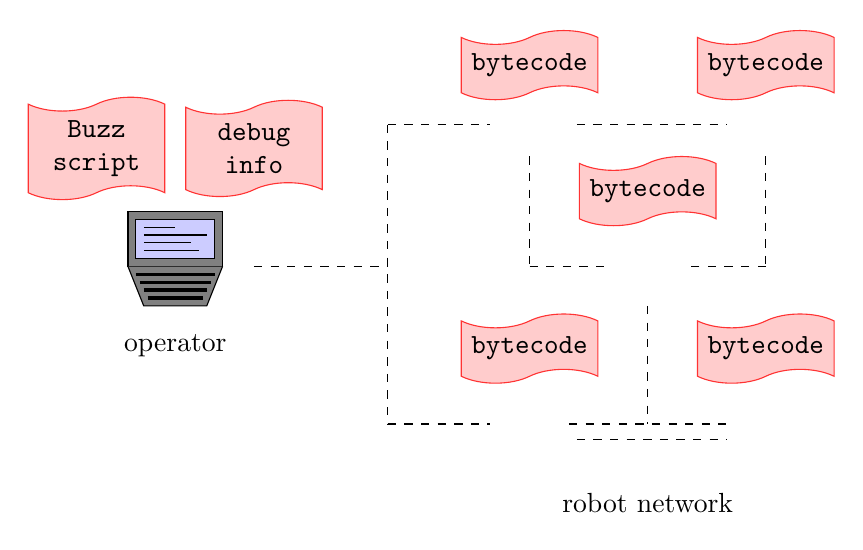
\begin{tikzpicture}[
  output/.style={draw=red!80,fill=red!20,tape,text width=1.5cm,align=center,font=\tt}
  ]

  % Script
  \node[output] at (-1cm,1.5cm) {Buzz\\script};

  % Debug information
  \node[output] at (1cm,1.5cm) {debug\\info};

  % Operator
  \filldraw[fill=black!50] (-6mm,  0mm) rectangle (6mm,7mm);
  \filldraw[fill=blue!20]  (-5mm,  1mm) rectangle (5mm,6mm);
  \draw (-4mm,5mm) -- (0mm,5mm);
  \draw (-4mm,4mm) -- (4mm,4mm);
  \draw (-4mm,3mm) -- (2mm,3mm);
  \draw (-4mm,2mm) -- (3mm,2mm);
  \filldraw[fill=black!50] (-6mm,  0mm) -- (-4mm,-5mm) -- (4mm, -5mm) -- (6mm,0mm);
  \draw[very thick] (-5  mm,-1mm) -- (5  mm,-1mm);
  \draw[very thick] (-4.5mm,-2mm) -- (4.5mm,-2mm);
  \draw[very thick] (-4  mm,-3mm) -- (4  mm,-3mm);
  \draw[very thick] (-3.5mm,-4mm) -- (3.5mm,-4mm);

  % Top robots
  \node[output,anchor=south] at (4.5cm,2.2cm) {bytecode};
  \aerial[fill=green!60!black]{(4cm,1.5cm)}{};
  \node[output,anchor=south] at (7.5cm,2.2cm) {bytecode};
  \aerial[fill=green!60!black]{(7cm,1.5cm)}{};

  % Middle robot
  \node[output,anchor=south] at (6cm,0.6cm) {bytecode};
  \wheeledmanip[fill=green!60!black]{(5.5cm,-0.5cm)}{};

  % Bottom robots
  \node[output,anchor=south] at (4.5cm,-1.4cm) {bytecode};
  \wheeled[fill=green!60!black]{(4cm,-2.5cm)}{};
  \node[output,anchor=south] at (7.5cm,-1.4cm) {bytecode};
  \wheeled[fill=green!60!black]{(7cm,-2.5cm)}{};

  % Communication lines
  \draw[dashed] (1  cm, 0  cm) -- (2.7cm, 0  cm) % operator to vert line
                (2.7cm, 1.8cm) -- (2.7cm,-2  cm) % vert line
                (2.7cm, 1.8cm) -- (4  cm, 1.8cm) % vert line to left top robot
                (5.1cm, 1.8cm) -- (7  cm, 1.8cm) % left to right top robot
                (2.7cm,-2  cm) -- (4  cm,-2  cm) % vert line to left bottom robot
                (5.1cm,-2.2cm) -- (7  cm,-2.2cm) % left to right bottom robot
                (4.5cm, 1.4cm) -- (4.5cm, 0  cm)
                (4.5cm, 0  cm) -- (5.5cm, 0  cm) % top left to center robot
                (7.5cm, 1.4cm) -- (7.5cm, 0  cm)
                (7.5cm, 0  cm) -- (6.5cm, 0  cm) % top right to center robot
                (6  cm,-0.5cm) -- (6  cm,-2  cm)
                (5  cm,-2  cm) -- (7  cm,-2  cm);

  % Labels
  \node at (0mm,-1cm) {operator};
  \node at (6cm,-3cm) {robot network};

\end{tikzpicture}

\end{document}